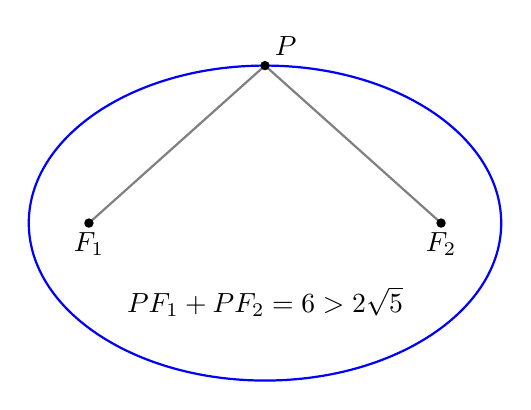
\begin{tikzpicture}[scale=1.0,>=stealth]
\draw[blue,thick] (0,0) ellipse (3 and 2);\draw[gray,thick] ({-sqrt(5)},0)--(0,2)--({sqrt(5)},0);\fill ({-sqrt(5)},0) circle (1.7pt) node[below] {$F_1$};\fill ({sqrt(5)},0) circle (1.7pt) node[below] {$F_2$};\fill (0,2) circle (1.7pt) node[above right] {$P$};\node at (0,-1) {$PF_1+PF_2=6>2\sqrt5$};
\end{tikzpicture}
